\documentclass[11pt, twoside, a4paper]{book}

    % chapters numbered without interruption (numbering through parts)
    \makeatletter\@addtoreset{chapter}{part}\makeatother
    \usepackage{graphicx}
    \graphicspath{ {./diagrams/images/} }
    \usepackage{pdflscape}
    \usepackage{color}
    \definecolor{Blue}{rgb}{0,0,0.9}
    \definecolor{Red}{rgb}{1,0,0}
    
    \begin{document}
    
        \title{Technical management processes of repository "foreign-language"}
        \author{Felipe Alves Matos Caggi}
        \maketitle
        
        \tableofcontents
        \newpage
        
        \chapter{INTRODUCTION}
        	
        	This document specifies the development process of the "foreign-language" system, providing the project manager with the necessary information for the planning and management of the project lifecycle.

            
            \section{Full view of this document}
            
                This introduction provides the information needed to make good use of this document, explaining its objectives and the conventions that have been adopted in the text, as well as contains a list of references to other related documents. The other sections present the specification of the "foreign-language" system and are organized as described below.
                
                \begin{itemize}
                
                    \item Section 2 - Project Planning Process: provides an overview of the system, characterizing the scope of the project management and technical activities, identifying process outputs, tasks and deliverables, establishing schedules for task conduct, including achievement criteria, and required resources	 to	accomplish tasks.
                    
                    \item Section 3 - Process Assessment and Control Process: specifies the status of the project, technical and process performance, helping ensure that the performance is according to plans and schedules, within projected budgets, to satisfy technical objectives.
                                        
                    \item Section 4 - Risk Management Process: provides information about risks of the project, describing process is to identify, analyze, treat and	monitor	the	risks continually.

                    \item Section 5 - Configuration Management Process: specifies all system elements what need to configuration management over the life cycle. Also, present the consistency management between a product and its associated configuration definition.
                    
                \end{itemize}						
                
            \section{Conventions, terms and abbreviations}
                
                The interpretation correct this document exige the knowledge of some conventionals and specific terms, that are describes next.	                
                
                \subsection{Identification of commits}
                	
                	\begin{center}
                		$[<Job Function ID Key\footnote{See section 2.2 for more details}>\_<Activity ID Key\footnote{See section 2.1 for more details}>\_<Commit Counter Per Job function>] <Description Commit>$
                	\end{center}
                
                \subsection{Identification of tags for baseline or releases}

					\begin{center}
						Baseline tag													

            			$[tgbl\_<Job Function ID Key>\_<Configuration Item Id Key For Management>\_<Tag Counter Per Item Of Configuration>]$
					\end{center}					                			

        			\begin{center}
		   				Release tag					        			
        			
            			$[tgrl\_<Job Function ID Key>\_<Configuration Item Id Key For Management>\_<Tag Counter Per Item Of Configuration>]$	
					\end{center}					                
					
            \section{References}
                    
                    Documents related to the "foreign-language" system and / or mentioned in the following sections:
            
        \chapter{PROJECT PLANNING PROCESS}
                	
        		\section{Project phases}
        		
					The development process adopted for this project has in its scope the following phases:
        			
        			\begin{enumerate}
        				
						\item Conception: is the first phase of the process, in which it seeks to raise the key requirements and understand the system comprehensively. The results of this phase are usually a requirement and risk document, a high-level use case listing, and a use case-based development timeline.
						\item Elaboration: this phase involves detailed system analysis, domain modeling and system design using the design patterns.
						\item Construction: includes a part of implementation and testing.
        				\item Transition: Upon ready, the system will be deployed replacing the current system of either manual or computerized.
        				
        			\end{enumerate}
        			
        			Subsections 2.2.1 and 2.2.4 present the details of the activities at each stage of the development process adopted.
	        		
	        		\subsection{Conception}

						The conception phase presents in its scope the following activities:	
							
	        			\begin{enumerate}
	        				
	        				\item $[busmdl]$ Business modeling (System overview)
	        					
								In this activity, all possible information about the system must be obtained. The product of this step will be \emph{system overview document}.        				
	        						
					        \item $[reqgat]$ Requirements Gathering
					        
					        	It corresponds to searching for all the possible information about the functions that the system must execute and the reticulations on which the system must operate. The product of this step will be the \emph{requirements document}, main component of the software design.
					        	
							\item $[reqaly]$ Requirements Analysis
							
								It serves to structure and detail the requirements so that they can be approached in the elaboration phase for the development of other elements such as use cases, classes, and interfaces.

							\item $[hlucse]$ High-level use cases
								
								In this activity it is necessary to identify the main use cases of the system. The use cases devel cover the main business activities linked to the system that will be developed.
								
	        			\end{enumerate}
	        			
    	    		\subsection{Elaboration}
    	    		
    	    			The elaboration phase presents in its scope the following activities:
	        			
	        			\begin{enumerate}
	        				
							\item Expansion of use cases								
							\item Determination of events and system responses
							\item Construction or refinement of the conceptual model
							\item Elaboration of operations contracts and system queries
							
	        			\end{enumerate}
	        			
        			\subsection{Construction}
        			
        			\subsection{Transicion}
        	
        	\section{Roles e responsibilities}
        	
				From the phases and activities defined in section 2.1, it was decided that this project will adopt the following roles for the members of the development team:
        		
				\begin{itemize}
        		        			
        			\item $[prjmn]$ Project manager: responsible for project management. The following activities are part of the project manager's scope of responsibilities:
        			
						\begin{enumerate}
							\item Define technical management processes.						
						\end{enumerate}					        			
        			
        			\item $[sysan]$ System analyst: it acts in the conception and elaboration phase, described in section 2.1.1 and 2.1.2. Responsible for the following activities:
        				\begin{enumerate}
        					\item Accomplish business modeling.
        					\item Raise system requirements.
        					\item Analyze requirements.
        					\item Define high-level use cases.
        					\item Expand use cases.
        				\end{enumerate}
        		
        			\item $[dsgnr]$ System designer: it acts in the elaboration phase described in section 2.1.2. Responsible for the following activities:
        				\begin{enumerate}
        					\item Determine system events and responses.
        					\item Build and refine conceptual model.
        					\item Elaboration of operating contract and system queries.
        				\end{enumerate}
        			
        			\item $[archt]$ Software architect
        			
        			\item $[progm]$ Programer
        			
        			\item $[testr]$ Tester
        			
        		\end{itemize}
                
              
			\begin{landscape}
				The figure below represents the mental map of the relationship between sections 2.1 and 2.2  
				\begin{figure}[!htb] 
					\center
   					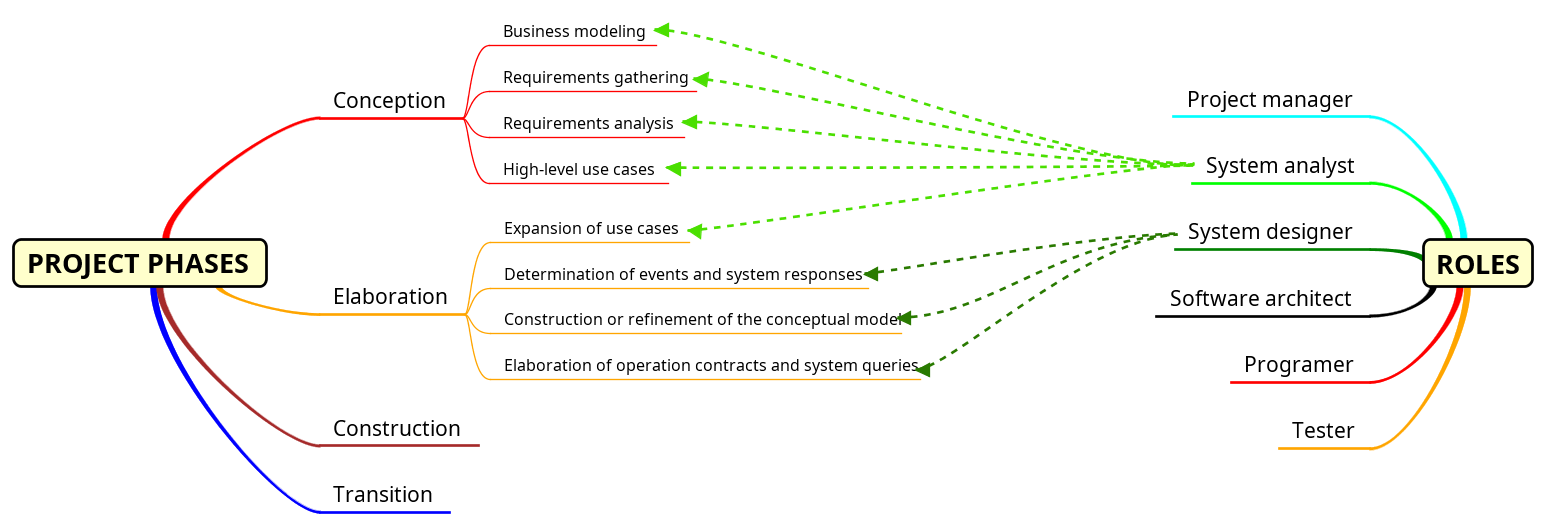
\includegraphics[scale=0.4,bb = 0 0 1545 525]{mindmap-phases_and_roles.png}
					\caption{Relationship between the activities of each phase of the project and the roles of the team members.}
				\end{figure}
			\end{landscape}		
        		
			\section{Infrastructure and services required}
				
				This section covers the infrastructure and services required for the development of the "foreign-language" system.
				
				\subsection{Computer-Aided Software Engineering}
					
					During project development, team members will use tools to aid in software engineering activities.
					
					Below are listed by category the tools required for the development of the "foreign language" system.

					\subsubsection{Documentation}
					
						\begin{itemize}
							\item Texmaker
						\end{itemize}
	
					\subsubsection{Edition}
						
						\begin{itemize}
							\item Astah
						\end{itemize}											
					
					\subsubsection{Hosting of code and / or documents}
        				
        				\begin{itemize}
        					\item GitHub
        				\end{itemize}
        				
					\subsubsection{Vesion control}
					
						\begin{itemize}
							\item Git
						\end{itemize}
						
			\section{Artifacts}
			
				Artifacts are final or intermediate work products that are produced and used during a project. Artifacts are used to capture and transmit project information.

				The artifacts adopted for this project are categorized into two types, document and model.
				
				\begin{itemize}
					\item A document, such as Business Case or Software Architecture Document 
					\item A template, such as the Use-Case Model or Design Template
				\end{itemize}
				
				\subsection{Documents}
				
					\begin{itemize}
						\item Software Development Plan
						\item Software Requiremtents Specification
						\item Software Architecture Document
						\item Implementation Model Document
						\item Software Test Plan
					\end{itemize}					
					
				\subsection{Models}
				
					\begin{itemize}
						\item UseCase Model
						\item Scenario
						\item UseCase Description						
						\item Analysis Model
						\item Design Model
						\item Implementation Model		
						\item Test Model
					\end{itemize}
			
			\section{Process and Artifact}
				
				It is important to highlight the artifacts generated in each phase of the project. The mind map below represents a relationship between the processes and the artifacts generated during each process.
				
				\begin{landscape}
				\textcolor{Red}{The figure below represents the mental map of the relationship between sections 2.1 and 2.2}
				\begin{figure}[!htb] 
					\center
   					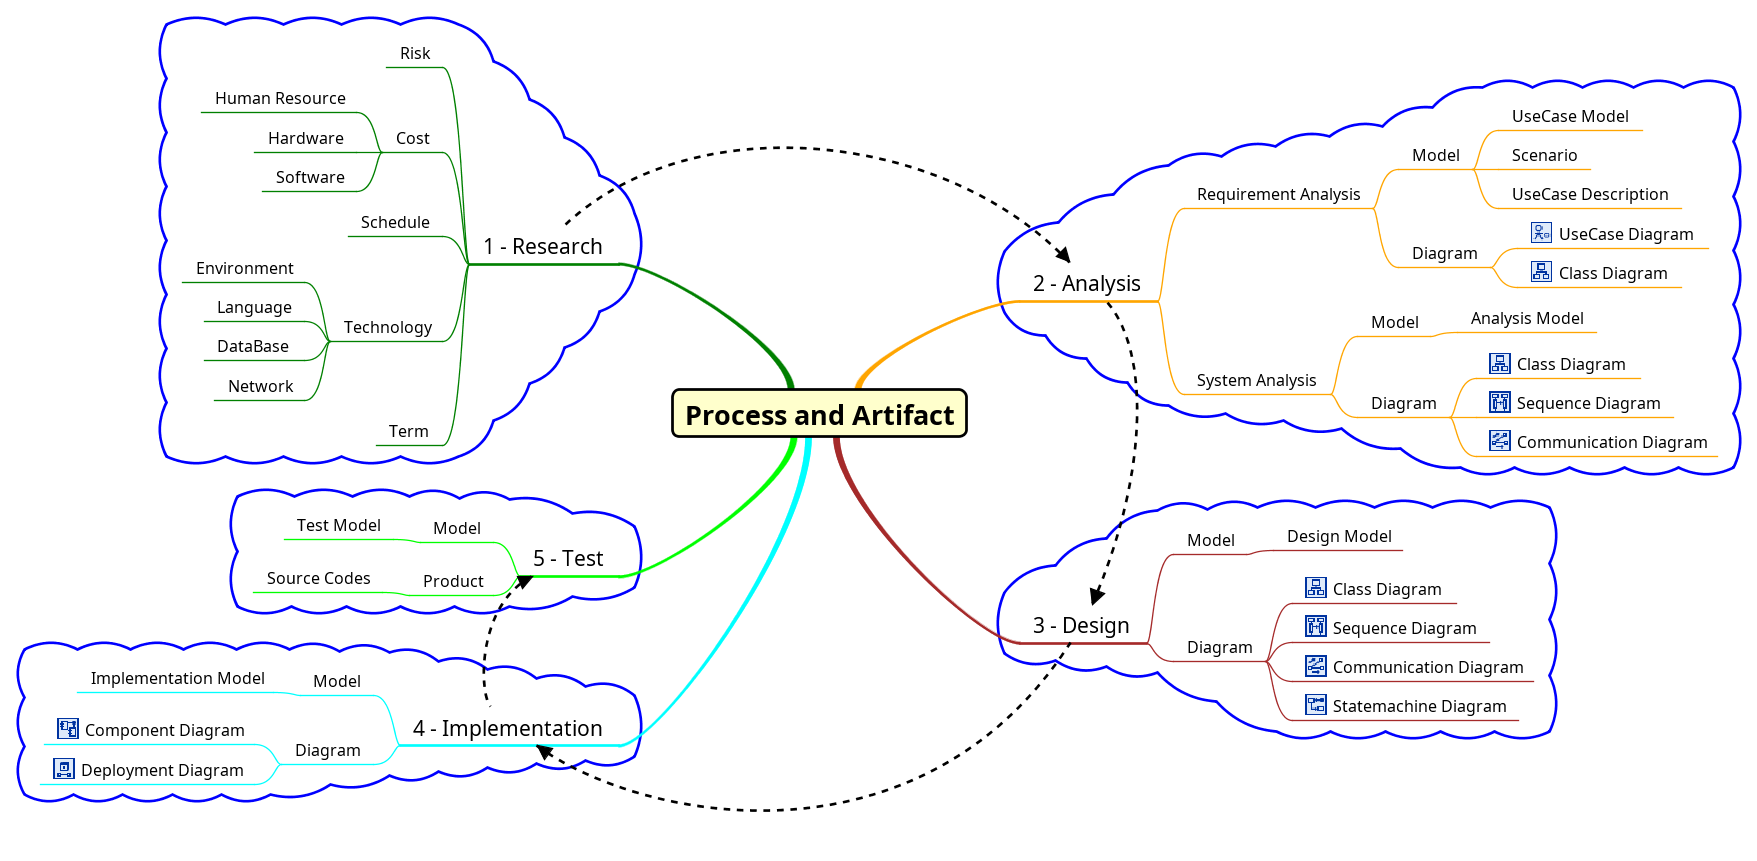
\includegraphics[scale=0.4,bb = 0 0 1545 525]{process-and-artifact.png}
					\textcolor{Red}{\caption{Relationship between the activities of each phase of the project and the roles of the team members.}}
				\end{figure}
			\end{landscape}	
        				
        \chapter{PROCESS ASSESSMENT AND CONTROL PROCESS}
                    
        \chapter{RISK MANAGEMENT PROCESS}
        
        \chapter{CONFIGURATION MANAGEMENT PROCESS}
    
    \end{document}